%   % !TEX root = ../../VIII,3_Rahmen-TeX_9-0.tex
%  
%   Signatur/Tex-Datei:	LH_37_05_019
%   RK-Nr. 	52278
%   Überschrift: 	Experiences à faire sur le mouvement
%   edlabels:			3
%   Diagramme: 		1
%
%
\selectlanguage{ngerman}
\frenchspacing
%
\begin{ledgroupsized}[r]{120mm}
\footnotesize
\pstart
\noindent\textbf{Überlieferung:}
\pend
\end{ledgroupsized}
%
\begin{ledgroupsized}[r]{114mm}
\footnotesize
\pstart \parindent -6mm
\makebox[6mm][l]{\textit{L}}%
Konzept:
LH~XXXVII~5~Bl.~19. 
Ein Blatt~4\textsuperscript{o}; 
Papiererhaltungsmaßnahmen;
Ränder beschnitten.
Eineinhalb Seiten.
\pend
\end{ledgroupsized}
%
\begin{ledgroupsized}[r]{114mm}
\footnotesize
\pstart
\parindent -6mm
\makebox[6mm][l]{\textit{E}}%
\cite{01056}\textsc{Fichant} 1994, S.~403\textendash405.
\pend%
\end{ledgroupsized}
%
%
%
\vspace{5mm}
\begin{ledgroup}
\footnotesize
\pstart
\noindent%
\textbf{Datierungsgründe:}
Beim vorliegenden Stück N.~\ref{52278} handelt es sich um einen Katalog geplanter Experimente über den elastischen und unelastischen Stoß mithilfe von Pendeln.
%
Der theoretische Rahmen und die Anlage der Experimente zeugen von dem bedeutenden Einfluss 
\protect\index{Namensregister}{\textso{Mariotte}, Edme, Seigneur de Chazeuil ca. 1620\textendash1684}%
Mariottes
auf Leibnizens Stoßlehre in der Zeit vor \textit{De corporum concursu}.
%
Die Entstehung des Stücks lässt sich durch folgende Umstände genauer einkreisen.%
\pend
%
\pstart
Die Nennung des Lederarbeiters und Erfinders 
\protect\index{Namensregister}{\textso{Lancker} 17.\ Jh.}Lancker in der Nr.\ (3) 
%
(S.~\refpassage{37_05_019_3a}{37_05_019_3b})
bietet einen sicheren Terminus post quem für N.~\ref{52278}.
%
Dieser hatte sein wasserundurchlässiges Leder Ende des Sommers 1677 in 
%
Paris\protect\index{Ortsregister}{Paris} vorgeführt 
%
(siehe den \cite{02048}Bericht im \cite{00157}\textit{Journal des Sçavans}, 31.\ Januar 1678, S.~39\textendash41).
%
Leibniz war bereits Ende September über diese Erfindung informiert, wovon sein \cite{02049}Brief an Jean Paul de La Roque vom 17.\ (27.) September 1677 (\textit{LSB} III,~2 N.~78, bes.\ S.~224) zeugt.
%
In den folgenden Monaten bat Leibniz verschiedene Pariser Korrespondenten, darunter
%
\protect\index{Namensregister}{\textso{Mariotte}, Edme, Seigneur de Chazeuil ca. 1620\textendash1684}%
Mariotte, wiederholt (und vergeblich) um ein Muster von 
\protect\index{Namensregister}{\textso{Lancker} 17.\ Jh.}Lanckers Leder
%
(\textit{LSB} I, 2, S.~294f. und 311; III, 2, S.~224, 308, 311, 353 und 908),
%
bis 
\protect\index{Namensregister}{\textso{Justel}, Henri 1620\textendash1693}Justel 
%
ihn im Juli 1679 \cite{02050}informierte, dass das wasserdichte Leder aus der Mode gekommen war
%
(\glqq n'est plus à la mode\grqq) und 
%
\protect\index{Namensregister}{\textso{Lancker} 17.\ Jh.}Lancker 
%
\protect\index{Ortsregister}{Paris}Paris verlassen hatte (\textit{LSB} I, 2, S.~502.26\textendash28).
%
\pend
%
\pstart
%
Ein Terminus ante quem für das Stück ergibt sich aus dem Vergleich mit einem 
%
wahrscheinlich im September 1677 entstandenen, vermutlich für \protect\index{Namensregister}{\textso{Bertet} (Berthet), Jean 1622\textendash1692}Jean Bertet bestimmten
%
\cite{02047}Brieffragment,	
%
worin Leibniz seine Fortschritte \glqq en matiere de mouvement\grqq\ seit der Pariser Zeit erwähnt.
%
Leibniz schreibt über die Stoß- und Bewegungsgesetze:
%
\glqq Je voy moyen d’en venir à bout demonstrativement, mais il faut faire premierement certaines experiences fondamentales que j’ay projettées. C’est ma maniere de dresser un Catalogue d’Experiences à faire, lors que j’examine quelque matiere de physique. Et ordinairement j’en fais un tel dénombrement que je puis asseurer que par le moyen de ces experiences on pourra trouver la cause ou la regle de ce dont il s’agit, demonstrativement, et non pas par Hypothese\grqq\ (\textit{LSB} II, 1 \lbrack2.\ Aufl.\rbrack, hier S.~572).
%
Die Identifizierung des hier genannten \glqq Catalogue d'Experiences à faire\grqq\ \glqq en matiere de mouvement\grqq\ mit dem 
%
vorliegenden Konzept N.~\ref{52278} erscheint sehr plausibel, wobei aus dem Brief nicht eindeutig hervorgeht, 
%
ob Leibniz diesen Katalog bereits ausgearbeitet oder lediglich die Experimente konzipiert hatte. 
%
Im ersten Fall würde der Brief selbst einen Terminus ante quem für N.~\ref{52278} bilden; 
%
auch im letzteren wäre eine zeitnahe Entstehung zum Brief für Bertet als wahrscheinlich anzusehen.
%
Daraus ergibt sich die vorgeschlagene Zeitspanne bis Oktober 1677, die auch dem mutmaßlichen Charakter der Datierung des Brieffragments Rechnung trägt.
%
\pend
%
%
\pstart
Mehrere Elemente und Aspekte der in N.~\ref{52278} geplanten Experimente verraten den Einfluss von
%
\protect\index{Namensregister}{\textso{Mariotte}, Edme, Seigneur de Chazeuil ca. 1620\textendash1684}Mariottes Verfahren,
%
am deutlichsten wohl die Verwendung von Pendeln und Kugeln (u.a.\ Lehmkugeln) zur Untersuchung des Stoßes.
%
Auch werden für \protect\index{Namensregister}{\textso{Mariotte}, Edme, Seigneur de Chazeuil ca. 1620\textendash1684}Mariotte 
%
charakteristische Thesen auf den Prüfstand gestellt: 
%
die Bewegung weicher Körper nach dem Stoß  in Nr.~(1) (\cite{00311}\title{Traité}, Première partie, Prop.~XI, S.~56\textendash60); 
%
die Erhaltung der Differenz der Bewegungsgrößen in Nr.~(2) (\cite{00311}a.a.O., Prop.~XII,  S.~60\textendash68); 
%
\protect\index{Namensregister}{\textso{Mariotte}, Edme, Seigneur de Chazeuil ca. 1620\textendash1684}Mariottes 
%
zentrale Annahme, dass der Stoß zweier Körper nicht von ihren eigenen, sondern nur von der respektiven Geschwindigkeit abhängt, in Nr.~(13) (\cite{00311}a.a.O., Prop.~III,  S.~25\textendash29).
%
Die letztgenannte Frage, \glqq si les vistesses respectives ou approchemens estant les mêmes, les percussions sont aussi également fortes\grqq\ (hier unter Nr.~13),
%
hatte Leibniz bereits in den kritischen Auszügen aus 
%
\protect\index{Namensregister}{\textso{Mariotte}, Edme, Seigneur de Chazeuil ca. 1620\textendash1684}Mariotte 
%
von März 1677 aufgeworfen (N.~\ref{57267_3}, S.~\refpassage{37_05_144-145_23a}{37_05_144-145_second_principe}).
%
Seine Untersuchung dieser Frage in den Stücken von Juni 1677 (N.~\ref{57269}, N.~\ref{57270} und N.~\ref{57271}) und seine Versuche, die \textit{vis ictus} im Verhältnis zur \textit{vis tota} der stoßenden Körper zu schätzen, 
%
hatten ihn damals zur Konzeption von einigen der hier detaillierter beschriebenen Experimente geführt 
%
(siehe den Schluss von N.~\ref{57271}, \textit{De vi ictus}, S.~\refpassage{37_05_159-160_10a}{37_05_159-160_10b}).
%
Diese Umstände stützen die vorgeschlagene Datierung von N.~\ref{52278} relativ zu \textit{De corporum concursu}:
%
In der Nr.~(13) von N.~\ref{52278} betrachtet Leibniz die Frage,
%
ob die \textit{vis ictus} nur von der respektiven Geschwindigkeit der Körper abhängt,
%
als eine offene, noch experimentell zu entscheidende,
%
gemäß dem im 
%
\cite{02047}Brief für 
%
\protect\index{Namensregister}{\textso{Bertet} (Berthet), Jean 1622\textendash1692}Bertet geschilderten Forschungsprogramm.
%
%
In der \textit{Scheda octava} von Januar 1678 erklärt er dieselbe Frage für im Sinne
%
\protect\index{Namensregister}{\textso{Mariotte}, Edme, Seigneur de Chazeuil ca. 1620\textendash1684}Mariottes
%
gelöst (S.~\refpassage{LH_37_05_086r_percussioeadem-3}{LH_37_05_086r_percussioeadem-2} von N.~\ref{dcc_08}).
%
Die \textit{Scheda decima} \textit{de corporum concursu}
%
(S.~\refpassage{LH_37_05_090r_satisfecimus-1}{LH_37_05_090r_satisfecimus-2} von N.~\ref{dcc_10})
%
stellt rückblickend fest, dass nunmehr die demonstrative Gewissheit der Theorie erreicht ist, 
%
wozu der \cite{02047}Brief für \protect\index{Namensregister}{\textso{Bertet} (Berthet), Jean 1622\textendash1692}Bertet
%
die Experimente als Mittel und vorbereitende Maßnahme angedacht hatte.
%
\pend
\end{ledgroup}
%
%
\selectlanguage{french}
\frenchspacing
% \newpage%
\vspace{8mm}
\pstart%
\normalsize%
\noindent%
\lbrack19~r\textsuperscript{o}\rbrack\
\pend %Wenn Überschrift/Diagramm
%
% Überschrift
\pstart
\centering
Experiences\protect\index{Sachverzeichnis}{experience} à faire sur le
%
\edlabel{37_05_019_1a}%
\edtext{}{% NEUER ABSATZ UND VARIANTEN – "(1) Si dans"
{\xxref%
{37_05_019_1a}{37_05_019_1b}}%
\lemma{mouvement}%
\Bfootnote{%
\textit{(1)}~(1) Si dans le concours de deux boules de terre glaise, il ne se perd rien de la force: ce qui n'est gueres croyable, \textbar\ à cause \textit{streicht Hrsg.}~\textbar\ %
 du son qu'elles font en se \textit{(2)}~(1) Si~\textit{L}}}%
mouvement
\pend
\vspace{\baselineskip}
%
\pstart
(1) Si%
\edlabel{37_05_019_1b}
%
lors qu'une boule de terre glaise\protect\index{Sachverzeichnis}{boule de terre glaise}\protect\index{Sachverzeichnis}{terre glaise} 
%
\edtext{ou cire\protect\index{Sachverzeichnis}{cire} en}{\lemma{}\Bfootnote{ou cire en \textit{erg.}~\textit{L}}} 
%
rencontre une autre en 
%
\edtext{repos, elles}{%
\lemma{}%
\Bfootnote{%
repos, \textbar\ si \textit{gestr.}~\textbar\ %
elles \textit{L}}}
%
vont par après ensemble avec la même quantité de mouvement.\protect\index{Sachverzeichnis}{quantité de mouvement}
%
Il faut essayer cecy 
%
\edtext{avec un long pendule,\protect\index{Sachverzeichnis}{pendule}}{\lemma{avec un}\Bfootnote{\textit{(1)}~pendule un peu long, \textit{(2)}~long pendule~\textit{L}}}
%
\edtext{et des}{\lemma{et}\Bfootnote{\textit{(1)}~une \textit{(2)}~des~\textit{L}}} 
%
boules\protect\index{Sachverzeichnis}{boule} assez grandes. Cela
%
\edtext{ne me}{\lemma{}\Bfootnote{ne me \textit{erg.}~\textit{L}}} 
%
paroist point vraisemblable, d'autant qu'elles font quelque bruit\protect\index{Sachverzeichnis}{bruit} en se frappant, 
%
et que l'applatissement\protect\index{Sachverzeichnis}{applatissement} témoigne qu'elles ont receu quelque mouvement\lbrack,\rbrack\ 
%
outre qu'il semble que la boule\protect\index{Sachverzeichnis}{boule} qui est en repos, ne laisse pas de resister
%
en quelque façon à une autre qui la veut mouvoir.
\pend 
%
\pstart
\edtext{(2) Quand}{\lemma{(2)}\Bfootnote{\textit{(1)}~Si \textit{(2)}~Quand~\textit{L}}} 
%
elles se rencontrent d'un mouvement 
%
\edtext{contraire,\protect\index{Sachverzeichnis}{mouvement contraire} il faut voir}{\lemma{contraire,}\Bfootnote{\textit{(1)}~sçavoir \textit{(2)}~il faut voir~\textit{L}}} 
%
s'il se perd la difference des quantités de mouvement.\protect\index{Sachverzeichnis}{difference des quantités de mouvement}
%
Cela est raisonable, il en faut observer le son.\protect\index{Sachverzeichnis}{son}
\pend 
%
\pstart
(3) On pourra faire des experiences\protect\index{Sachverzeichnis}{experience} avec des sacs pleins d'eau\protect\index{Sachverzeichnis}{sac plein d'eau} et bien bouchez.
%
Cela reussira mieux qu'avec de la terre glaise,\protect\index{Sachverzeichnis}{terre glaise} 
%
\edlabel{37_05_019_3a}%	zw. Referenzierung
le cuir\protect\index{Sachverzeichnis}{cuir} de 
%
\protect\index{Namensregister}{\textso{Lancker} 17.\ Jh.}M.~Lancker y sera propre.%
\edlabel{37_05_019_3b}
%
L'eau\protect\index{Sachverzeichnis}{eau} ne fait gueres de ressort,\protect\index{Sachverzeichnis}{ressort} à ce que je croy.
\pend 
%
\pstart
(4) Pour 
%
\edtext{faire avec des corps à ressort\protect\index{Sachverzeichnis}{corps à ressort} des experiences\protect\index{Sachverzeichnis}{experience} aisées à distinguer par le menu, on}{\lemma{faire}%
\Bfootnote{
\textit{(1)}~des experiences aisées à distinguer par le menu avec des corps à ressort, %
\textit{(2)}~des experiences avec des corps %
\textit{(3)}~avec \lbrack...\rbrack\ on~\textit{L}}}
%
se pourra servir des balons enflés;\protect\index{Sachverzeichnis}{ballon enflé} car on verra
visiblement comment ils s'applatiront,
%
\edtext{et en un}{%
\lemma{}%
\Bfootnote{%
et \textbar\ en \textit{erg.}~\textbar\ un~\textit{L}}}
%
mot toute l’oeconomie et tout le 
%
\edtext{détail de}{%
\lemma{détail}%
\Bfootnote{%
\textit{(1)}~du pro %
\textit{(2)}~de~\textit{L}}}
%
l’ordre que la nature observe en cecy.
\pend
%
\pstart
(5) Pour separer ce qui fait l'effort,\protect\index{Sachverzeichnis}{effort} d’avec ce qui recoit le 
%
\edtext{choc,\protect\index{Sachverzeichnis}{choc} ou}{%
\lemma{choc,}%
\Bfootnote{%
\textit{(1)}~et %
\textit{(2)}~ou~\textit{L}}}
%
qui fait ressort,\protect\index{Sachverzeichnis}{ressort} on suspendra des poids au bas des balons\protect\index{Sachverzeichnis}{ballon} ou boules\protect\index{Sachverzeichnis}{boule}
%
qui se rencontrent: ou même on les attachera
%
\edtext{fermement au}{%
\lemma{fermement}%
\Bfootnote{%
\textit{(1)}~au plu %
\textit{(2)}~au~\textit{L}}}
%
dessous ou au dessus du balon à une verge.
\pend 
%
\pstart
(6) On fera qu'un corps en rencontre deux \edtext{ou d'avantage}{\lemma{}\Bfootnote{ou d'avantage \textit{erg.}~\textit{L} }} 
%
tout à la fois, placés 
%
\edtext{l'un auprès}{\lemma{l'un}\Bfootnote{\textit{(1)}~autre \textit{(2)}~auprès~\textit{L}}}
%
ou derriere l'autre.
\pend 
%
\pstart
(7) Item \edtext{on disposera}{\lemma{on}\Bfootnote{\textit{(1)}~fera \ \textit{(2)}~disposera~\textit{L}}} 
%
les pendules\protect\index{Sachverzeichnis}{pendule} en sorte qu'ils
%
\edtext{se rencontrent}{\lemma{se}\Bfootnote{\textit{(1)}~disposent \textit{(2)}~rencontrent~\textit{L}}}
%
obliquement. 
\pend 
%
\pstart
(8) On fera les experiences des rencontres\protect\index{Sachverzeichnis}{experience des rencontres} avec des cloches\protect\index{Sachverzeichnis}{cloche} ou 
%
\edtext{sonnettes\protect\index{Sachverzeichnis}{sonnette} ou}{\lemma{sonnettes}\Bfootnote{\textit{(1)}~, pour juger \textit{(2)}~ou~\textit{L}}} 
%
chordes tendues,\protect\index{Sachverzeichnis}{chorde tendue} pour juger 
%
par le son\protect\index{Sachverzeichnis}{son} de la force 
%
de la percussion,\protect\index{Sachverzeichnis}{force de la percussion} en tant qu'elle doit 
%
\edtext{estre distinguée}{\lemma{estre}\Bfootnote{\textit{(1)}~separée de \textit{(2)}~distinguée~\textit{L}}}
%
de la force de tout le mouvement.\protect\index{Sachverzeichnis}{force de tout le mouvement}%
%
%
\pend 
%
\pstart
(9) On fera en sorte que les corps se rencontrent autrement que suivant leurs centres de 
%
\edlabel{37_05_019_2a}%
\edtext{}{% NEUER ABSATZ UND VARIANTEN – gravité. (10) On
{\xxref%
{37_05_019_2a}{37_05_019_2b}}%
\lemma{gravité}%
\Bfootnote{%
\textit{(1)}~On se \textit{(2)}~(10) On se~\textit{L}\ }}%
gravité.\protect\index{Sachverzeichnis}{centre de gravité}
\pend
%
\pstart
(10) On se%
\edlabel{37_05_019_2b}
%
servira de toutes sortes de figures.
\pend 
%
\pstart
(11) Toutes ces experiences\protect\index{Sachverzeichnis}{experience} seront faites avec des 
%
\edtext{corps d'une}{%
\lemma{corps}%
\Bfootnote{%
\textit{(1)}~fort %
\textit{(2)}~d'une~\textit{L}}}
%
grandeur et pesanteur considerable, et avec de longs pendules,\protect\index{Sachverzeichnis}{pendule} à
%
\edtext{fin que ce}{\lemma{fin que}\Bfootnote{\textit{(1)}~l'erreur qui peut \textit{(2)}~ce \textit{L }\ }} 
%
que la resistence de
%
\edtext{l'air,\protect\index{Sachverzeichnis}{air}\protect\index{Sachverzeichnis}{resistence de l'air} le}{\lemma{l'air}\Bfootnote{\textit{(1)}~et de l \textit{(2)}~, le~\textit{L}}} 
%
frottement\protect\index{Sachverzeichnis}{frottement} de la corde,\protect\index{Sachverzeichnis}{corde} et choses semblables y peuvent contribuer ne soit gueres considerable.
\pend 
%
\pstart
\lbrack19~v\textsuperscript{o}\rbrack\
(12) Les boules de terre glaise\protect\index{Sachverzeichnis}{boule de terre glaise}\protect\index{Sachverzeichnis}{terre glaise}
%
ne sont pas si propres aux experiences\protect\index{Sachverzeichnis}{experience} que
%
les ballons enflés d'eau,\protect\index{Sachverzeichnis}{ballon enflé d'eau} parce que ces ballons\protect\index{Sachverzeichnis}{ballon} ne s'attachent pas,
%
au lieu que l'attachement de cette terre molle\protect\index{Sachverzeichnis}{terre molle} sert beaucoup à empecher
%
la separation des boules,\protect\index{Sachverzeichnis}{boule} et à changer ce qui arriveroit sans cela.
\pend 
%
\pstart
(13) Il faut examiner bien exactement, si les vistesses respectives\protect\index{Sachverzeichnis}{vistesse respective} ou approchemens estant
%
les mêmes, les percussions\protect\index{Sachverzeichnis}{percussion} sont aussi également fortes. 
%
C'est à dire si deux enfans suspendus d'un filet,\protect\index{Sachverzeichnis}{enfant suspendu d'un filet} et se rencontrant avec la même vistesse 
%
sentiront autant de douleur,\protect\index{Sachverzeichnis}{douleur} soit que l'un d'entre eux soit en repos, ou qu'ils aillent l'un contre l'autre. 
%
Mais pour bien examiner cecy, il faut se servir des boules\protect\index{Sachverzeichnis}{boule} et mesurer 
%
\edtext{leur applatissement,\protect\index{Sachverzeichnis}{applatissement} et}{\lemma{}\Bfootnote{applatissement, \textbar \ qu'elles ont visiblement, \textit{gestr.}~\textbar\ et~\textit{L}}}
%
leur son.
%
L'applatissement\protect\index{Sachverzeichnis}{applatissement} se mesurera ainsi:
%
une boule\protect\index{Sachverzeichnis}{boule} estant mouillée ou tachée de quelque couleur, 
%
et l'autre ne l'estant point, on verra en celle que ne l'estoit point jusqu'à où alloit l'applatissement.\protect\index{Sachverzeichnis}{applatissement}
\pend
%
%
\vspace{2.0em} %%%%%%%%% Diagramm 1
\centerline{%
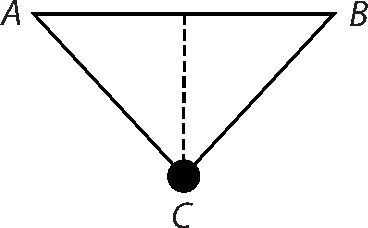
\includegraphics[width=0.3\textwidth]{%
gesamttex/edit_VIII,3/images/LH_37_05_019_d_019v.pdf%
}} 
\vspace{0.5em}
\centerline{%
\lbrack\textit{Fig.~1}\rbrack%
}
% \newpage%
\vspace{1.5em}
%
%
\pstart
(14) Il \edtext{faut qu'un}{\lemma{faut}\Bfootnote{\textit{(1)}~que les pend \textit{(2)}~qu'un~\textit{L}}} 
%
pendule\protect\index{Sachverzeichnis}{pendule} \edtext{\textit{C}}{%
\lemma{}%
\Bfootnote{%
\textit{C} %
\textit{erg.\ L}%
}}
%
soit suspendu à deux fils \textit{AC}.\textit{BC}.\ et l'axe de l'agitation\protect\index{Sachverzeichnis}{axe de l'agitation} sera \textit{AB}.%
\pend
%
\pstart
(15) Si
\edtext{la percussion\protect\index{Sachverzeichnis}{percussion}}{%
\lemma{la}%
\Bfootnote{%
\textit{(1)}~même %
\textit{(2)}~percussion~\textit{L}}}
%
estoit la même, ce seroit vray aussi à l'égard des corps mols\protect\index{Sachverzeichnis}{corps mou}; et par 
%
\edtext{consequent les}{%
\lemma{consequent}%
\Bfootnote{%
\textit{(1)}~la per %
\textit{(2)}~les~\textit{L}}}
%
corps mols\protect\index{Sachverzeichnis}{corps mou} dont un avoit esté en 
%
\edtext{repos, ne}{\lemma{repos,}\Bfootnote{\textit{(1)}~n'iroient \textit{(2)}~ne~\textit{L}}}
%
conserveroient pas toute la force\protect\index{Sachverzeichnis}{force} avec le choc, et il s'en perdroit aussi bien, que 
%
lors qu'ils se rencontrent d'un mouvement contraire.\protect\index{Sachverzeichnis}{mouvement contraire}
%
Mais considerant maintenant la chose un peu plus 
%
\edtext{attentivement, je doute si la force de}{\lemma{attentivement,}%
\Bfootnote{\textit{(1)}~je croy que non obstant que 
\textit{(2)}~je doute si \textit{(a)}~la percussion des corps mols fut la même
\textit{(b)}~\textbar\ si \textit{streicht Hrsg.}~\textbar\ la force 
\textit{(aa)}~se doit perd \textit{(bb)}~de~\textit{L}}} 
%
la percussion\protect\index{Sachverzeichnis}{force de la percussion} se doit perdre en eux.
\pend
\count\Afootins=1200%
\count\Bfootins=1200%
\count\Cfootins=1200